\chapter{布尔代数}
\intro{逻辑推理的代数化——布尔代数用一套简洁的公理描述"真"与"假"的运算规则，是数字电路设计的数学基础。}

\section{布尔代数的定义}

\subsection{公理化定义}

\begin{mydefinition}{布尔代数}
一个\textbf{布尔代数}是代数系统 \((B,+,\cdot,{}',0,1)\)，其中 \(B\) 是至少包含两个元素 \(0\) 和 \(1\) 的集合，\(+\) 和 \(\cdot\) 是 \(B\) 上的二元运算，\({}'\) 是 \(B\) 上的一元运算，满足以下公理。
\end{mydefinition}

对任意 \(a,b,c\in B\)：

\begin{enumerate}[label=\textbf{B\arabic*}:,leftmargin=*]
    \item 交换律：\(a+b=b+a\)
    \item[$\text{B}1'$] \(a\cdot b = b\cdot a\)
    \item 结合律：\(a+(b+c)=(a+b)+c\)
    \item[$\text{B}2'$] \(a\cdot(b\cdot c)=(a\cdot b)\cdot c\)
    \item 幺元：\(a+0=a\)
    \item[$\text{B}3'$] \(a\cdot 1 = a\)
    \item 排中律：\(a+a'=1\)
    \item[$\text{B}4'$] 矛盾律：\(a\cdot a'=0\)
    \item 分配律：\(a+(b\cdot c)=(a+b)\cdot(a+c)\)
    \item[$\text{B}5'$] \(a\cdot(b+c)=(a\cdot b)+(a\cdot c)\)
\end{enumerate}

其中 \(0\) 称为\textbf{零元}（下界），\(1\) 称为\textbf{幺元}（上界），\(a'\) 称为 \(a\) 的\textbf{补元}。运算 \(+\) 称为\textbf{布尔和}（OR），\(\cdot\) 称为\textbf{布尔积}（AND）。

\begin{myTheorem}{对偶原理}
布尔代数的公理具有完全对称的\textbf{对偶性}——将 \(+\) 与 \(\cdot\) 互换、\(0\) 与 \(1\) 互换，所得命题仍成立。
\end{myTheorem}

\subsection{亨廷顿公理体系}

数学家E.\,V.~Huntington在1904年给出了更精简的公理系统：

\begin{enumerate}[label=\textbf{H\arabic*}:,leftmargin=*]
    \item \(a+b=b+a\)
    \item \((a+b)+c=a+(b+c)\)
    \item \(a+b\) 由 \(a,b\) 唯一确定
    \item 存在 \(0,1\) 使得 \(a+0=a\)，且对每个 \(a\) 存在 \(a'\) 满足 \(a+a'=1\)
\end{enumerate}

亨廷顿还证明：若 \(B\) 有至少两个元素，这组公理足以推出所有布尔代数定理。

\subsection{作为有补分配格的布尔代数}

\begin{mydefinition}{格论视角的布尔代数}
布尔代数是一个\textbf{有补的分配格}。格中有最大元 \(1\) 和最小元 \(0\)，每个元素 \(a\) 有补元 \(a'\)：\(a\vee a'=1\) 且 \(a\wedge a'=0\)。在分配格中，补元若存在则唯一。
\end{mydefinition}

偏序关系：\(a \leq b \iff a+b=b \iff a\cdot b = a\)。

\begin{center}
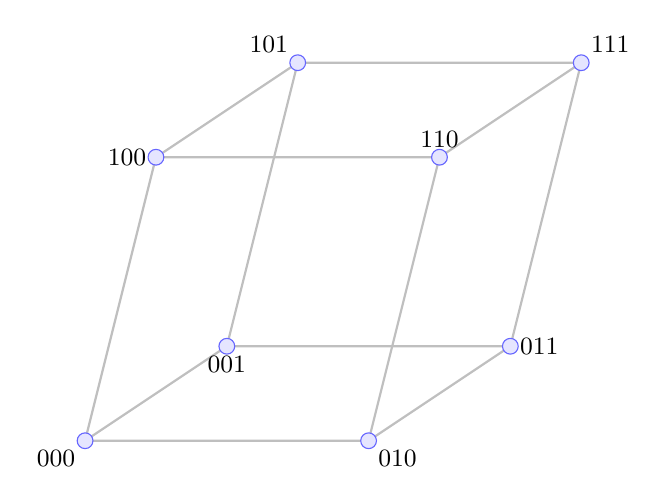
\begin{tikzpicture}[scale=1.2]
\tikzset{
    dmCubeNode/.style={circle,draw=blue!60,fill=blue!10,minimum size=2mm,inner sep=1pt},
    dmCubeLabel/.style={font=\small}
}
% 3D cube representing Boolean lattice of 3 variables
\coordinate (A) at (0,0);    % 000
\coordinate (B) at (1.5,1);  % 001
\coordinate (C) at (3,0);    % 010
\coordinate (D) at (4.5,1);  % 011
\coordinate (E) at (0.75,3); % 100
\coordinate (F) at (2.25,4); % 101
\coordinate (G) at (3.75,3); % 110
\coordinate (H) at (5.25,4); % 111

\draw[gray!50,thick] (A) -- (B) -- (D) -- (C) -- (A);
\draw[gray!50,thick] (E) -- (F) -- (H) -- (G) -- (E);
\draw[gray!50,thick] (A) -- (E);
\draw[gray!50,thick] (B) -- (F);
\draw[gray!50,thick] (C) -- (G);
\draw[gray!50,thick] (D) -- (H);

\node[dmCubeNode] at (A) {};
\node[dmCubeLabel,below left] at (A) {\(000\)};
\node[dmCubeNode] at (B) {};
\node[dmCubeLabel,below] at (B) {\(001\)};
\node[dmCubeNode] at (C) {};
\node[dmCubeLabel,below right] at (C) {\(010\)};
\node[dmCubeNode] at (D) {};
\node[dmCubeLabel,right] at (D) {\(011\)};
\node[dmCubeNode] at (E) {};
\node[dmCubeLabel,left] at (E) {\(100\)};
\node[dmCubeNode] at (F) {};
\node[dmCubeLabel,above left] at (F) {\(101\)};
\node[dmCubeNode] at (G) {};
\node[dmCubeLabel,above] at (G) {\(110\)};
\node[dmCubeNode] at (H) {};
\node[dmCubeLabel,above right] at (H) {\(111\)};
\end{tikzpicture}
\captionof{figure}{三元布尔代数的立方体格结构——每个顶点对应一个三元组，顶点间的边表示相邻关系。}
\end{center}

\subsection{重要例子}

\begin{table}[H]
\centering
\begin{tabular}{lccccc}
\toprule
布尔代数 & 元素 & \(+/\vee\) & \(\cdot/\wedge\) & \({}'\) & \(0\) / \(1\) \\
\midrule
二值布尔代数 \(\mathbb{B}\) & \(\{0,1\}\) & OR & AND & NOT & 0 / 1 \\
集合代数 & \(\mathcal{P}(X)\) & \(\cup\) & \(\cap\) & 补集 & \(\varnothing\) / \(X\) \\
命题逻辑 & \(\{F,T\}\) & \(\lor\) & \(\land\) & \(\neg\) & F / T \\
除数格 & \(\{d\mid d\mid n\}\) & \(\lcm\) & \(\gcd\) & \(n/d\) & 1 / \(n\) \\
\bottomrule
\end{tabular}
\end{table}

\section{布尔代数的基本性质}

\subsection{幂等律}

\begin{myformula}
\[
a + a = a, \qquad a\cdot a = a
\]
\end{myformula}

\begin{proof}[证明]
以 \(a+a=a\) 为例：
\[
\begin{aligned}
a &= a + 0                     && \text{(B3: 幺元)} \\
  &= a + (a \cdot a')          && \text{(B4$'$: 矛盾律)} \\
  &= (a + a)\cdot(a + a')      && \text{(B5: 分配律)} \\
  &= (a + a)\cdot 1            && \text{(B4: 排中律)} \\
  &= a + a                     && \text{(B3$'$: 幺元)}
\end{aligned}
\]
另一式由对偶原理可得。
\end{proof}

\subsection{零律}

\begin{myformula}
\[
a + 1 = 1, \qquad a\cdot 0 = 0
\]
\end{myformula}

\begin{proof}[证明]
以 \(a+1=1\) 为例：
\[
\begin{aligned}
a + 1 &= (a+1) \cdot 1                       && \text{(B3$'$)} \\
      &= (a+1)\cdot(a+a')                    && \text{(B4)} \\
      &= a + (1\cdot a')                     && \text{(B5: 分配律)} \\
      &= a + a'                              && \text{(B3$'$)} \\
      &= 1                                   && \text{(B4)}
\end{aligned}
\]
\end{proof}

\subsection{吸收律}

\begin{myformula}
\[
a + (a\cdot b) = a, \qquad a\cdot(a+b) = a
\]
\end{myformula}

\begin{proof}[证明]
以 \(a+(a\cdot b)=a\) 为例：
\[
\begin{aligned}
a + (a\cdot b) &= (a\cdot 1) + (a\cdot b)    && \text{(B3$'$)} \\
               &= a\cdot(1+b)                && \text{(B5$'$: 分配律)} \\
               &= a\cdot 1                   && \text{(零律)} \\
               &= a                          && \text{(B3$'$)}
\end{aligned}
\]
\end{proof}

\subsection{补元的唯一性}

\begin{myTheorem}{补元唯一性}
布尔代数中，每个元素 \(a\) 的补元是唯一的。
\end{myTheorem}

\begin{proof}[证明]
设 \(b\) 和 \(c\) 都是 \(a\) 的补元，即 \(a+b=1\)，\(a\cdot b=0\) 且 \(a+c=1\)，\(a\cdot c=0\)。则：
\[
\begin{aligned}
b &= b\cdot 1 = b\cdot(a+c) = (b\cdot a)+(b\cdot c) \\
  &= (a\cdot b)+(b\cdot c) = 0+(b\cdot c) = (a\cdot c)+(b\cdot c) \\
  &= (c\cdot a)+(c\cdot b) = c\cdot(a+b) = c\cdot 1 = c
\end{aligned}
\]
\end{proof}

\subsection{德摩根律}

\begin{myformula}
\[
(a+b)' = a'\cdot b', \qquad (a\cdot b)' = a' + b'
\]
\end{myformula}

\begin{proof}[证明]
以 \((a+b)' = a'\cdot b'\) 为例。验证 \(a'\cdot b'\) 是 \(a+b\) 的补元：
\[
\begin{aligned}
(a+b)+(a'\cdot b') &= [(a+b)+a']\cdot[(a+b)+b'] \\
                   &= [1+b]\cdot[a+1] = 1\cdot 1 = 1 \\[4pt]
(a+b)\cdot(a'\cdot b') &= [a\cdot(a'\cdot b')] + [b\cdot(a'\cdot b')] \\
                        &= [0\cdot b'] + [0\cdot a'] = 0 + 0 = 0
\end{aligned}
\]
由补元唯一性，\(a'\cdot b' = (a+b)'\)。
\end{proof}

\subsection{双重否定律}

\[
(a')' = a
\]

\begin{proof}[证明]
\(a'\) 的补元满足 \(a'+(a')'=1\) 且 \(a'\cdot(a')'=0\)；同时 \(a'+a=1\) 且 \(a'\cdot a=0\)。由补元唯一性得 \((a')'=a\)。
\end{proof}

\subsection{性质总表}

\begin{table}[H]
\centering
\small
\begin{tabular}{lll}
\toprule
名称 & OR形式 & AND形式 \\
\midrule
幂等律 & \(a+a=a\) & \(a\cdot a=a\) \\
交换律 & \(a+b=b+a\) & \(a\cdot b=b\cdot a\) \\
结合律 & \(a+(b+c)=(a+b)+c\) & \(a\cdot(b\cdot c)=(a\cdot b)\cdot c\) \\
分配律 & \(a+(b\cdot c)=(a+b)\cdot(a+c)\) & \(a\cdot(b+c)=a\cdot b+a\cdot c\) \\
同一律 & \(a+0=a\) & \(a\cdot 1=a\) \\
零律 & \(a+1=1\) & \(a\cdot 0=0\) \\
吸收律 & \(a+(a\cdot b)=a\) & \(a\cdot(a+b)=a\) \\
德摩根律 & \((a+b)'=a'\cdot b'\) & \((a\cdot b)'=a'+b'\) \\
双重否定律 & \((a')'=a\) & \((a')'=a\) \\
对合律 & \(0'=1\) & \(1'=0\) \\
\bottomrule
\end{tabular}
\end{table}

\section{布尔函数}

\subsection{布尔函数的定义}

\begin{mydefinition}{布尔函数}
从布尔代数 \(B^n\) 到 \(B\) 的一个映射 \(f: B^n \to B\) 称为一个 \(n\) 元布尔函数。在最基本的情形，\(B=\{0,1\}\)。
\end{mydefinition}

\begin{mydefinition}{布尔表达式}
由布尔变量 \(x_1,x_2,\dots,x_n\) 通过运算 \(+,\cdot,{}'\) 和常量 \(0,1\) 构成的表达式称为布尔表达式。每个布尔表达式定义一个布尔函数。
\end{mydefinition}

例如：\(f(x,y,z)=xy+x'z+yz'\) 定义了一个三元布尔函数。

\begin{myTheorem}{布尔函数的数量}
\(n\) 个变量的布尔函数共有 \(2^{2^n}\) 个。
\end{myTheorem}

\begin{proof}[证明]
\(n\) 个布尔变量有 \(2^n\) 种输入组合。对每种组合，输出可取 \(0\) 或 \(1\)。因此共有 \(2^{2^n}\) 种输出模式。
\end{proof}

\begin{table}[H]
\centering
\begin{tabular}{cccr}
\toprule
\(n\) & 输入组合数 \(2^n\) & 布尔函数个数 \(2^{2^n}\) & 示例 \\
\midrule
1 & 2 & 4 & NOT, 恒等, 恒0, 恒1 \\
2 & 4 & 16 & AND, OR, XOR, NAND \\
3 & 8 & 256 & 多数表决、全加器 \\
4 & 16 & 65536 & 各种组合电路 \\
\bottomrule
\end{tabular}
\end{table}

\subsection{极小项与极大项}

\begin{mydefinition}{极小项与极大项}
\begin{itemize}
    \item \textbf{极小项}：\(n\) 个变量的一个布尔积，每个变量（或其补）恰好出现一次，如 \(x\,y'\,z\)。
    \item \textbf{极大项}：\(n\) 个变量的一个布尔和，每个变量（或其补）恰好出现一次，如 \(x+y'+z\)。
\end{itemize}
\end{mydefinition}

每个极小项在恰好一种赋值下为 \(1\)，每个极大项在恰好一种赋值下为 \(0\)。

\begin{myTheorem}{标准形定理}
每个非零布尔函数可唯一表示为极小项之和（SOP）；每个非1的布尔函数可唯一表示为极大项之积（POS）。
\end{myTheorem}

\section{布尔表达式的化简}

\subsection{代数化简法}

常用化简技巧：

\begin{enumerate}[label=\arabic*.]
    \item \textbf{合并}：\(ab+ab' = a(b+b') = a\cdot 1 = a\)
    \item \textbf{吸收}：\(a+ab = a(1+b) = a\)
    \item \textbf{消去}：\(a+a'b = a+b\)（因 \((a+a')(a+b)=1\cdot(a+b)=a+b\)）
    \item \textbf{一致项}：\(ab+a'c+bc = ab+a'c\)（一致项 \(bc\) 可消去）
\end{enumerate}

\begin{example}
化简 \(F = AB + A'C + BC\)：
\[
\begin{aligned}
F &= AB + A'C + BC\cdot 1 \\
  &= AB + A'C + BC(A+A') \\
  &= AB + A'C + ABC + A'BC \\
  &= AB(1+C) + A'C(1+B) \\
  &= AB + A'C
\end{aligned}
\]
\end{example}

\subsection{卡诺图}

卡诺图是Maurice Karnaugh于1953年提出的可视化化简工具。

\subsubsection{2变量卡诺图}

\begin{center}
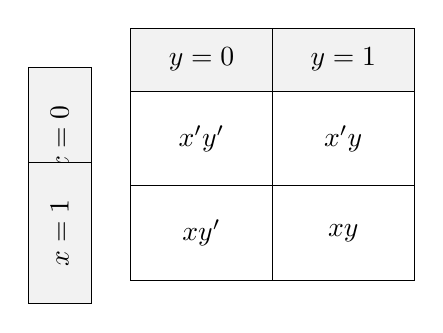
\begin{tikzpicture}
\tikzset{
    dmKmapCell/.style={rectangle,draw=black,minimum width=1.8cm,minimum height=1.2cm,align=center},
    dmKmapHead/.style={rectangle,draw=black,minimum width=1.8cm,minimum height=0.8cm,align=center,fill=gray!10},
}
\node[dmKmapHead] (h00) at (0,1.6) {\(y=0\)};
\node[dmKmapHead] (h01) at (1.8,1.6) {\(y=1\)};
\node[dmKmapHead,rotate=90] (h10) at (-1.8,0.6) {\(x=0\)};
\node[dmKmapHead,rotate=90] (h11) at (-1.8,-0.6) {\(x=1\)};

\node[dmKmapCell] (c00) at (0,0.6) {\(x'y'\)};
\node[dmKmapCell] (c01) at (1.8,0.6) {\(x'y\)};
\node[dmKmapCell] (c10) at (0,-0.6) {\(xy'\)};
\node[dmKmapCell] (c11) at (1.8,-0.6) {\(xy\)};
\end{tikzpicture}
\captionof{figure}{2变量卡诺图——相邻方格仅一位变量不同。}
\end{center}

\subsubsection{3变量卡诺图}

\begin{center}
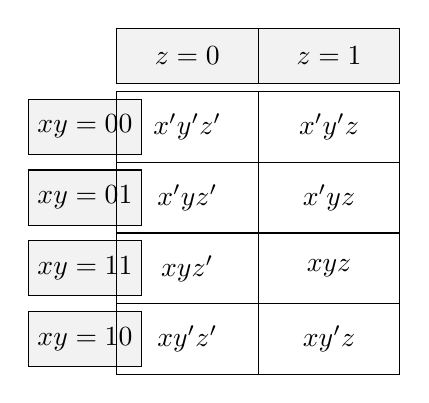
\begin{tikzpicture}
\tikzset{
    dmKmap3/.style={rectangle,draw=black,minimum width=1.8cm,minimum height=0.9cm,align=center},
    dmKmap3Head/.style={rectangle,draw=black,minimum width=1.8cm,minimum height=0.7cm,align=center,fill=gray!10},
}
\node[dmKmap3Head] at (0,1.8) {\(z=0\)};
\node[dmKmap3Head] at (1.8,1.8) {\(z=1\)};

\node[dmKmap3Head,minimum width=0.8cm] at (-1.3,0.9) {\(xy=00\)};
\node[dmKmap3Head,minimum width=0.8cm] at (-1.3,0) {\(xy=01\)};
\node[dmKmap3Head,minimum width=0.8cm] at (-1.3,-0.9) {\(xy=11\)};
\node[dmKmap3Head,minimum width=0.8cm] at (-1.3,-1.8) {\(xy=10\)};

\node[dmKmap3] at (0,0.9) {\(x'y'z'\)};
\node[dmKmap3] at (1.8,0.9) {\(x'y'z\)};
\node[dmKmap3] at (0,0) {\(x'yz'\)};
\node[dmKmap3] at (1.8,0) {\(x'yz\)};
\node[dmKmap3] at (0,-0.9) {\(xyz'\)};
\node[dmKmap3] at (1.8,-0.9) {\(xyz\)};
\node[dmKmap3] at (0,-1.8) {\(xy'z'\)};
\node[dmKmap3] at (1.8,-1.8) {\(xy'z\)};
\end{tikzpicture}
\captionof{figure}{3变量卡诺图——采用格雷码排列 \(00\to01\to11\to10\)。}
\end{center}

\subsubsection{4变量卡诺图}

\begin{center}
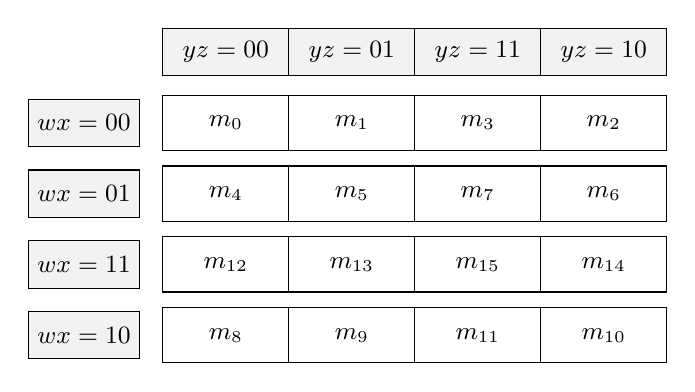
\begin{tikzpicture}
\tikzset{
    dmKmap4/.style={rectangle,draw=black,minimum width=1.6cm,minimum height=0.7cm,align=center,font=\small},
    dmKmap4Head/.style={rectangle,draw=black,minimum width=1.6cm,minimum height=0.6cm,align=center,fill=gray!10,font=\small},
}
\node[dmKmap4Head] at (0.8,1.8) {\(yz=00\)};
\node[dmKmap4Head] at (2.4,1.8) {\(yz=01\)};
\node[dmKmap4Head] at (4.0,1.8) {\(yz=11\)};
\node[dmKmap4Head] at (5.6,1.8) {\(yz=10\)};

\node[dmKmap4Head,minimum width=0.8cm] at (-1.0,0.9) {\(wx=00\)};
\node[dmKmap4Head,minimum width=0.8cm] at (-1.0,0) {\(wx=01\)};
\node[dmKmap4Head,minimum width=0.8cm] at (-1.0,-0.9) {\(wx=11\)};
\node[dmKmap4Head,minimum width=0.8cm] at (-1.0,-1.8) {\(wx=10\)};

\foreach \x/\y/\t in {
    0.8/0.9/m_0, 2.4/0.9/m_1, 4.0/0.9/m_3, 5.6/0.9/m_2,
    0.8/0/m_4, 2.4/0/m_5, 4.0/0/m_7, 5.6/0/m_6,
    0.8/-0.9/m_{12}, 2.4/-0.9/m_{13}, 4.0/-0.9/m_{15}, 5.6/-0.9/m_{14},
    0.8/-1.8/m_8, 2.4/-1.8/m_9, 4.0/-1.8/m_{11}, 5.6/-1.8/m_{10}
} {
    \node[dmKmap4] at (\x,\y) {\(\t\)};
}
\end{tikzpicture}
\captionof{figure}{4变量卡诺图——\(m_k\) 表示第 \(k\) 个极小项。}
\end{center}

\textbf{卡诺图化简步骤}：

\begin{enumerate}
    \item 将函数填入卡诺图（1的格子填1，0的填0）
    \item 用尽可能大的矩形圈住所有的1，每个矩形大小为 \(2^k\) 个格子
    \item 矩形可跨越边界（循环相邻）；圈数尽量少
    \item 每个圈对应一项——变量取值不变的保留，发生变化的消去
\end{enumerate}

\subsubsection{无关项}

实际电路设计中，某些输入组合永远不会出现，或输出不影响结果。这些情况用 \(\times\) 或 \(d\) 标记，称为\textbf{无关项}。化简时，无关项可当做0或1，怎么有利于化简就怎么取。

\subsection{Quine-McCluskey算法}

当 \(n\geq 5\) 时，卡诺图不再适用。Q-M算法是系统化的表格化简方法。

\vspace{4pt}
\textbf{算法核心思想}：
\begin{enumerate}
    \item 列出所有极小项的二进制形式
    \item 按含1的个数分组
    \item 在相邻组间寻找海明距离为1的项合并，差异位标记为``-''
    \item 重复直到无法继续合并
    \item 构建质蕴含表，选取覆盖所有极小项的最少质蕴含项
\end{enumerate}

复杂度：最坏情况指数级（NP-hard问题）。

\section{逻辑门电路}

\subsection{基本逻辑门}

\vspace{4pt}
\begin{center}
\begin{tikzpicture}[scale=0.85]
\tikzset{
    dmGateNOT/.style={draw=red!60!black,fill=red!5,minimum width=1.6cm,minimum height=0.8cm,align=center},
    dmGateAND/.style={draw=blue!60!black,fill=blue!5,minimum width=1.6cm,minimum height=0.8cm,align=center},
    dmGateOR/.style={draw=green!40!black,fill=green!5,minimum width=1.6cm,minimum height=0.8cm,align=center},
    dmGateNAND/.style={draw=orange!80!black,fill=orange!5,minimum width=1.6cm,minimum height=0.8cm,align=center},
    dmGateNOR/.style={draw=purple!60!black,fill=purple!5,minimum width=1.6cm,minimum height=0.8cm,align=center},
    dmGateXOR/.style={draw=brown!60!black,fill=brown!5,minimum width=1.6cm,minimum height=0.8cm,align=center},
}

\node[dmGateNOT] (not) at (0,5) {NOT\\[-2pt]\(F=A'\)};
\node[dmGateAND] (and) at (0,3.5) {AND\\[-2pt]\(F=AB\)};
\node[dmGateOR] (or) at (0,2) {OR\\[-2pt]\(F=A+B\)};
\node[dmGateNAND] (nand) at (8,5) {NAND\\[-2pt]\(F=(AB)'\)};
\node[dmGateNOR] (nor) at (8,3.5) {NOR\\[-2pt]\(F=(A+B)'\)};
\node[dmGateXOR] (xor) at (8,2) {XOR\\[-2pt]\(F=A\oplus B\)};
\node[dmGateXOR] (xnor) at (8,0.5) {XNOR\\[-2pt]\(F=(A\oplus B)'\)};

\draw[dmEdge] (not.west) ++(-0.5,0) -- (not.west);
\draw[dmEdge] (and.west) ++(-0.5,0.15) -- (and.west) node[pos=0,left]{\scriptsize\(A\)};
\draw[dmEdge] (and.west) ++(-0.5,-0.15) -- (and.west) node[pos=0,left]{\scriptsize\(B\)};
\draw[dmEdge] (or.west) ++(-0.5,0.15) -- (or.west);
\draw[dmEdge] (or.west) ++(-0.5,-0.15) -- (or.west);
\draw[dmEdge] (nand.west) ++(-0.5,0.15) -- (nand.west);
\draw[dmEdge] (nand.west) ++(-0.5,-0.15) -- (nand.west);
\draw[dmEdge] (nor.west) ++(-0.5,0.15) -- (nor.west);
\draw[dmEdge] (nor.west) ++(-0.5,-0.15) -- (nor.west);
\draw[dmEdge] (xor.west) ++(-0.5,0.15) -- (xor.west);
\draw[dmEdge] (xor.west) ++(-0.5,-0.15) -- (xor.west);
\draw[dmEdge] (xnor.west) ++(-0.5,0.15) -- (xnor.west);
\draw[dmEdge] (xnor.west) ++(-0.5,-0.15) -- (xnor.west);
\end{tikzpicture}
\captionof{figure}{七种基本逻辑门符号及其布尔表达式。}
\end{center}

\subsection{真值表}

\begin{table}[H]
\centering
\begin{tabular}{cc|cccccc}
\toprule
\(A\) & \(B\) & AND & OR & NAND & NOR & XOR & XNOR \\
\midrule
0 & 0 & 0 & 0 & 1 & 1 & 0 & 1 \\
0 & 1 & 0 & 1 & 1 & 0 & 1 & 0 \\
1 & 0 & 0 & 1 & 1 & 0 & 1 & 0 \\
1 & 1 & 1 & 1 & 0 & 0 & 0 & 1 \\
\bottomrule
\end{tabular}
\caption{基本逻辑门的真值表}
\end{table}

\subsection{功能完备性}

\begin{mydefinition}{功能完备集}
一组逻辑门称为\textbf{功能完备}的，如果仅用这组门就能实现任意布尔函数。
\end{mydefinition}

\begin{myTheorem}{NAND完备性}
\{NAND\} 单独就是功能完备的。用NAND可实现：
\[
\text{NOT }A = A\text{ NAND }A,\quad
A\text{ AND }B = (A\text{ NAND }B)\text{ NAND }(A\text{ NAND }B)
\]
\[
A\text{ OR }B = (A\text{ NAND }A)\text{ NAND }(B\text{ NAND }B)
\]
\end{myTheorem}

\begin{center}
\begin{tikzpicture}[scale=0.9]
\tikzset{
    dmNandConv/.style={draw=orange!80!black,fill=orange!5,minimum width=1.6cm,minimum height=0.7cm,align=center,font=\small},
}
\node[dmNandConv] (n1) at (0,4) {NAND};
\node[dmBox] (l1) at (3,4) {NOT};
\draw[dmEdge] (n1) -- (l1);
\draw[dmEdge] (n1.north west) ++(-0.5,0.1) -- (n1.north west);
\draw[dmEdge] (n1.south west) ++(-0.5,-0.1) -- (n1.south west);
\node[anchor=west] at (4.2,4) {\(A\text{ NAND }A = A'\)};

\node[dmNandConv] (n2a) at (0,2.5) {NAND};
\node[dmNandConv] (n2b) at (3,2.5) {NAND};
\node[dmBox] (l2) at (6,2.5) {AND};
\draw[dmEdge] (n2a.east) ++(0.1,0.15) -- (n2a.east);
\draw[dmEdge] (n2b.west) ++(-0.1,0.15) -- (n2b.west);
\draw[dmEdge] (n2a.east) ++(0.1,-0.15) -- (n2a.east);
\draw[dmEdge] (n2b.west) ++(-0.1,-0.15) -- (n2b.west);
\draw[dmEdge] (n2b) -- (l2);
\node[anchor=west] at (7.2,2.5) {\((A\text{ NAND }B)\text{ NAND }(A\text{ NAND }B) = AB\)};

\node[dmNandConv] (n3a) at (0,1) {NAND};
\node[dmNandConv] (n3b) at (0.5,0) {NAND};
\node[dmNandConv] (n3c) at (3,0.5) {NAND};
\node[dmBox] (l3) at (6,0.5) {OR};
\draw[dmEdge] (n3a) -- (n3c);
\draw[dmEdge] (n3b) -- (n3c);
\draw[dmEdge] (n3c) -- (l3);
\node[anchor=west] at (7.2,0.5) {\((A\text{ NAND }A)\text{ NAND }(B\text{ NAND }B) = A+B\)};
\end{tikzpicture}
\captionof{figure}{用NAND门实现NOT、AND、OR：NAND门单独构成功能完备集。}
\end{center}

\subsection{加法器电路}

\textbf{半加器}：\(S = A\oplus B\)，\(C = A\cdot B\)。

\textbf{全加器}：
\[
S = A \oplus B \oplus C_{\text{in}},\qquad
C_{\text{out}} = AB + AC_{\text{in}} + BC_{\text{in}}
\]

\begin{center}
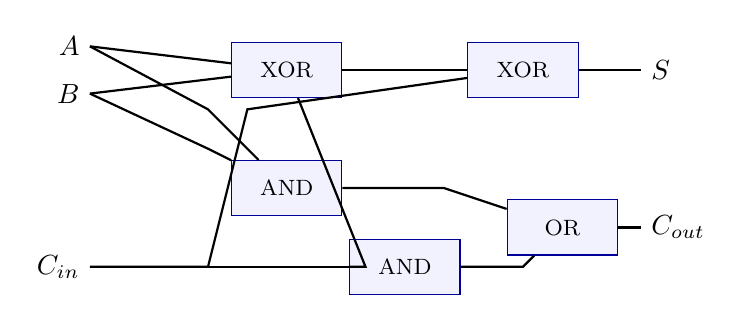
\begin{tikzpicture}[scale=1.0]
\tikzset{
    dmGateSym/.style={draw=blue!60!black,fill=blue!5,minimum width=1.4cm,minimum height=0.7cm,align=center,font=\footnotesize},
    dmWire/.style={thick},
}
\node[dmGateSym] (xor1) at (0,0) {XOR};
\node[dmGateSym] (xor2) at (3,0) {XOR};
\node[dmGateSym] (and1) at (0,-1.5) {AND};
\node[dmGateSym] (and2) at (1.5,-2.5) {AND};
\node[dmGateSym] (or1) at (3.5,-2) {OR};

\draw[dmWire] (-2.5,0.3) node[left]{\(A\)} -- (xor1);
\draw[dmWire] (-2.5,-0.3) node[left]{\(B\)} -- (xor1);
\draw[dmWire] (xor1) -- (xor2);
\draw[dmWire] (-2.5,-2.5) node[left]{\(C_{\text{in}}\)} -- (-1,-2.5) -- (-0.5,-0.5) -- (xor2);
\draw[dmWire] (-2.5,0.3) -- (-1,-0.5) -- (and1);
\draw[dmWire] (-2.5,-0.3) -- (-1,-1) -- (and1);
\draw[dmWire] (and1) -- (2,-1.5) -- (or1);
\draw[dmWire] (-1,-2.5) -- (and2);
\draw[dmWire] (xor1) -- (1,-2.5) -- (and2);
\draw[dmWire] (and2) -- (3,-2.5) -- (or1);
\draw[dmWire] (or1) -- (4.5,-2) node[right]{\(C_{\text{out}}\)};
\draw[dmWire] (xor2) -- (4.5,0) node[right]{\(S\)};
\end{tikzpicture}
\captionof{figure}{全加器电路图——由2个XOR门、2个AND门和1个OR门构成。}
\end{center}

多个全加器级联可实现多位二进制加法器。

\section{编程实现}

\begin{mycode}{布尔函数真值表生成}
\begin{lstlisting}[language=Python]
from itertools import product
from typing import Callable, List

def truth_table(variables: List[str],
                func: Callable[..., int]) -> str:
    """生成布尔函数的真值表"""
    n = len(variables)
    header = " | ".join(variables) + " | F"
    lines = [header, "-" * len(header)]
    for values in product([0, 1], repeat=n):
        result = func(*values)
        row = " | ".join(str(v) for v in values) + f" | {result}"
        lines.append(row)
    return "\n".join(lines)

def majority(a: int, b: int, c: int) -> int:
    """多数表决器：F = AB + AC + BC"""
    return (a & b) | (a & c) | (b & c)

print(truth_table(["A", "B", "C"], majority))
\end{lstlisting}
\end{mycode}

\begin{mycode}{Quine-McCluskey算法}
\begin{lstlisting}[language=Python]
from typing import List, Set, Dict

def minterm_to_binary(m: int, n_vars: int) -> str:
    return format(m, f'0{n_vars}b')

def hamming_distance(s1: str, s2: str) -> int:
    return sum(c1 != c2 for c1, c2 in zip(s1, s2))

def combine_terms(t1: str, t2: str) -> str:
    result = list(t1)
    for i, (c1, c2) in enumerate(zip(t1, t2)):
        if c1 != c2:
            result[i] = '-'
    return ''.join(result)

def qm_algorithm(minterms: List[int], n_vars: int) -> Set[str]:
    implicants = set(minterm_to_binary(m, n_vars) for m in minterms)
    while True:
        groups: Dict[int, List[str]] = {}
        for imp in implicants:
            ones = imp.count('1')
            groups.setdefault(ones, []).append(imp)
        new_implicants, used = set(), set()
        sorted_keys = sorted(groups.keys())
        for i in range(len(sorted_keys) - 1):
            k1, k2 = sorted_keys[i], sorted_keys[i + 1]
            if k1 + 1 != k2: continue
            for t1 in groups[k1]:
                for t2 in groups[k2]:
                    if hamming_distance(t1, t2) == 1:
                        combined = combine_terms(t1, t2)
                        new_implicants.add(combined)
                        used.add(t1); used.add(t2)
        prime = implicants - used
        if not new_implicants:
            return implicants
        implicants = new_implicants | prime

def term_to_expression(term: str, variables: List[str]) -> str:
    parts = []
    for i, (ch, var) in enumerate(zip(term, variables)):
        if ch == '1': parts.append(var)
        elif ch == '0': parts.append(f"{var}'")
    return ''.join(parts) if parts else '1'

# 示例
minterms = [0,1,2,4,5,6,8,9,12,13,14]
primes = qm_algorithm(minterms, 4)
for p in primes:
    print(f"  {p} -> {term_to_expression(p, ['w','x','y','z'])}")
\end{lstlisting}
\end{mycode}

\begin{mycode}{逻辑电路仿真器}
\begin{lstlisting}[language=Python]
from itertools import product
from typing import Dict, List, Tuple, Callable

class LogicSim:
    """组合逻辑电路仿真器"""
    def __init__(self):
        self.gates: List[Tuple[str, List[str], str, Callable]] = []
        self.signals: Dict[str, int] = {}

    def set_input(self, name: str, value: int):
        self.signals[name] = value

    def add_not(self, input_name: str, output_name: str):
        self.gates.append(("NOT", [input_name], output_name, lambda a: 1 - a))

    def add_and(self, in1: str, in2: str, output_name: str):
        self.gates.append(("AND", [in1, in2], output_name, lambda a, b: a & b))

    def add_or(self, in1: str, in2: str, output_name: str):
        self.gates.append(("OR", [in1, in2], output_name, lambda a, b: a | b))

    def add_xor(self, in1: str, in2: str, output_name: str):
        self.gates.append(("XOR", [in1, in2], output_name, lambda a, b: a ^ b))

    def simulate(self) -> Dict[str, int]:
        for _, inputs, output, func in self.gates:
            args = [self.signals[name] for name in inputs]
            self.signals[output] = func(*args)
        return dict(self.signals)

    def truth_table(self, input_names: List[str],
                    output_name: str) -> str:
        results = []
        header = " | ".join(input_names) + f" | {output_name}"
        results.append(header)
        results.append("-" * len(header))
        for values in product([0, 1], repeat=len(input_names)):
            self.signals.clear()
            for name, val in zip(input_names, values):
                self.signals[name] = val
            self.simulate()
            row = " | ".join(str(v) for v in values)
            row += f" | {self.signals[output_name]}"
            results.append(row)
        return "\n".join(results)

sim = LogicSim()
sim.add_xor("A", "B", "S")
sim.add_and("A", "B", "C")
print("半加器真值表：")
print(sim.truth_table(["A", "B"], "S"))
\end{lstlisting}
\end{mycode}

\section*{本章小结}

\begin{table}[H]
\centering
\begin{tabular}{lp{10cm}}
\toprule
概念 & 核心要点 \\
\midrule
布尔代数 & 公理化代数系统 \((B,+,\cdot,{}',0,1)\)，也是有补分配格 \\
对偶原理 & 交换 \(+\leftrightarrow\cdot\)、\(0\leftrightarrow1\) 得对偶命题 \\
布尔函数 & \(n\) 变量共有 \(2^{2^n}\) 个布尔函数 \\
标准形 & SOP（极小项之和）与POS（极大项之积）唯一表示 \\
卡诺图 & \(\leqslant 4\) 变量可视化化简；无关项可灵活利用 \\
Q-M算法 & 系统化表格化简，适合编程实现 \\
逻辑门 & NAND门单独功能完备 \\
加法器 & 半加器 \(S=A\oplus B\)；全加器可级联 \\
\bottomrule
\end{tabular}
\end{table}
